\documentclass{article}
% \usepackage{cTex}
\usepackage{float}
\usepackage{enumerate}
\usepackage{amsmath,amsfonts,amssymb,amsthm}
\usepackage{geometry,graphicx,subfigure}
\usepackage{cite,hyperref}
\usepackage{color}
\usepackage{caption,booktabs,boxedminipage}
\hypersetup{colorlinks=true,linkcolor=black}

\usepackage{listings}
\lstset{language=c++}
\lstset{breaklines}
\lstset{extendedchars=false}
\lstset{numbers=left, numberstyle=\small}
\lstset{keywordstyle=\color{blue}\bfseries}
\lstset{identifierstyle=\bf}
\lstset{numberstyle=\color[RGB]{0,192,192}}
\lstset{commentstyle=\it\color[RGB]{96,96,96}}
\lstset{stringstyle=\rmfamily\slshape\color[RGB]{128,0,0}}
\lstset{frame=shadowbox}
\lstset{basicstyle=\small\ttfamily}
\lstset{morekeywords={constructor,string,uint256,msg,now,modifier,address,function,payable,external,internal, selfdestruct}}
\geometry{left = 2cm, right = 2cm, top = 2cm, bottom = 2cm}
\linespread{1.0}

\usepackage[ruled,lined,boxed,linesnumbered]{algorithm2e}
\newtheorem{theorem}{Theorem}[section]
\newtheorem{lemma}[theorem]{Lemma}
\newtheorem{proposition}[theorem]{Proposition}
\newtheorem{corollary}[theorem]{Corollary}
\newtheorem{exercise}{Exercise}[section]
% \newtheorem*{solution}{Solution}
\newenvironment{solution}{\begin{proof}[Solution]\renewcommand{\qedsymbol}{}}{\end{proof}}

\title{Smart Contract }
\author{Li Jingyu\quad 517030910318\\Liu Du\quad 517030910346}
% \date{517030910318}
\begin{document}
\maketitle

\newcommand{\vecb}[2]{\boldsymbol{#1}^{(#2)}}
\newcommand{\code}[1]{{\ttfamily #1}}

\tableofcontents

\section{Introduction}

\subsection{Project Overview}
\label{sec:proj}
In this project, we design and implement an transparent and interactive crowdfunding distributed application (DApp) based on smart contract of the Ethereum Blockchain. The DApp has the following functionality:
\begin{itemize}
    \item \textbf{Basic crowdfunding}: Project manager can raise fund for the project. Anyone who supports the project are the backers and shall have the reward when the project succeeds. The project only begins if raised funding is larger than a threshold.
    \item \textbf{Insurance mechanism}: The project manager cannot get all the raised funding at once. Instead, The project is divided into several phases and only a portion of the funding is usable for one particular phase. The remaining money serves as the insurance. Once a phase is complete, backers can vote whether to continue the project or withdraw their money from the insurance.
    \item \textbf{Tradable share}: Backers can sell their share in the project for any price (as long as someone else would like to buy). They can sell at a higher price for profits or lower price if they lose confidence and want to reduce their loss.
\end{itemize}

we build a test chain and ...

\subsection{Block Chain and Ethereum}

\subsection{Smart Contract and DApp}
The term smart contract has been used over the years to describe a wide variety of different things. In the 1990s, cryptographer Nick Szabo coined the term and defined it as “a set of promises, specified in digital form, including protocols within which the parties perform on the other promises.” Since then, the concept of smart contracts has evolved, especially after the introduction of decentralized blockchain platforms with the invention of Bitcoin in 2009. In the context of Ethereum, the term is actually a bit of a misnomer, given that Ethereum smart contracts are neither smart nor legal contracts, but the term has stuck. In this book, we use the term “smart contracts” to refer to \textbf{immutable computer programs that run deterministically in the context of an Ethereum Virtual Machine} as part of the Ethereum network protocol. i.e., on the decentralized Ethereum world computer.

A decentralized application (DApp) is a computer application that runs on a distributed computing system. DApps have been popularized by distributed ledger technologies (DLT) such as the Ethereum Blockchain, where DApps are often referred to as smart contracts. DApps have their backend code running on a decentralized peer-to-peer network, as opposed to typical applications where the backend code is running on centralized servers. A DApp can have frontend code and user interfaces written in any language that can make calls to its backend. Furthermore, its frontend can be hosted on decentralized storage such as Swarm or IPFS.

\section{Writing Smart Contract}
\subsection{Solidity}
Solidity is an object-oriented, high-level language specifically for writing smart contracts. It was influenced by C++, Python and JavaScript and is designed to target the Ethereum Virtual Machine (EVM). Solidity is statically typed, supports inheritance, libraries and complex user-defined types among other features. We choose Solidity as our language for writing smart contracts 

\subsection{Requirement Specification}
As introduced in section \ref{sec:proj}, we have three main functionalities for our crowdfunding DApp: basic crowdfunding, insurance mechanism and tradable share. Here we specify these functionalities in detail.

For the basic crowdfunding, we need:
\begin{itemize}
    \item \code{support()}: People support money to the project and become backers
    \item \code{retract()}: Before the fund raising phase ends, if backers wants to give up their support, they can retract all their money
    \item \code{refund()}: After the fund raising phase ends, if raised money is less than the goal, all money is refunded to backers and the project will not begin.
\end{itemize}

For the insurance mechanism, we need:
\begin{itemize}
    \item \code{postRequest()}: The project manager can post request to enter the next phase and get the next portion of money. He/She must also post the current progress for reference (except for the first one). A ballot is simultaneously created. 
    \item \code{vote()}: Any backer can vote for the request or against. And in case a backer does not vote, every backer has a positive vote by default.
    \item \code{completeReq()}: After the ballot is due, the manager should be continue the project with more money or suspend the project  based on the result of the ballot.
\end{itemize}

For the tradable share, we need:
\begin{itemize}
    \item \code{postSale()}: a backer can sell part or all of his/her share at any price. If all the share is sold, he/she will be removed from the backer list.
    \item \code{cancelSale()}: If no one has purchased the share and the seller wants to continue to hold the share , he/she can cancel the sale.
    \item \code{buyShare()}: A buyer, whether he/she is a backer or not, can buy the share at the given price. Then the buyer would be eligible for the vote and the reward just as other backers.
\end{itemize}

\subsection{Design}
In Solidity, each contract is a class. So based on the above analysis, we can write the smart contracts in an inheritance manner, as shown in Figure~\ref{fig:design}.

\begin{figure}[H]
    \centering
    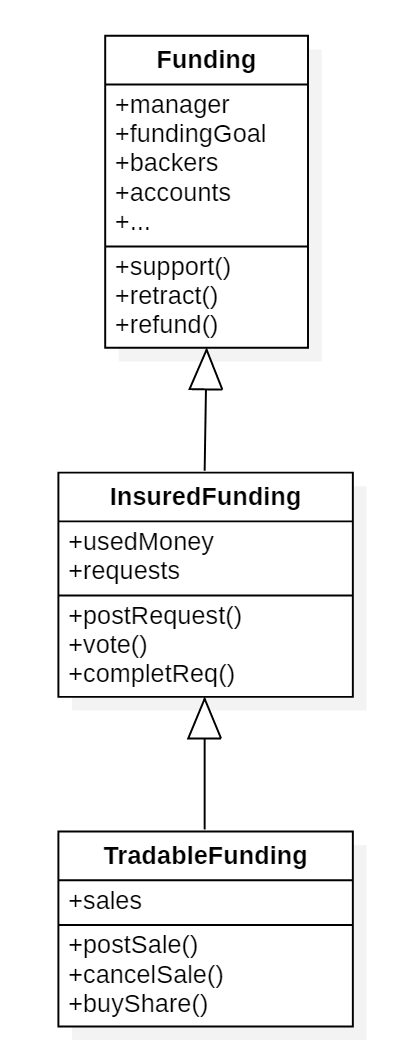
\includegraphics[width=0.3\linewidth]{fig/design.png}
    \caption{Design Diagram}
    \label{fig:design}
\end{figure}

\subsection{Implementation}
\subsubsection{Modifiers}
Since the core function of smart contracts is to deal with transaction, there are many modifiers of methods (of a contract) specifying the constraint of whether the transaction can be carried out. Using modifier makes the logic of the code unambiguous and clear. There are several kinds of modifiers:
\begin{itemize}
    \item \code{Payable} is a keyword in Solidity denoting that this method supports transaction from the message sender to the destination contract (where the method belongs to). The message sender and the transferred money is not explicitly specified in the parameter list. Instead, they are stored in the global variable \code{msg.sender} and \code{msg.value}. The transaction also does not need any explicit statement in the method.
    \item Access modifiers. There are four access modifiers: \code{public}, \code{private}, \code{external}, \code{internal}. Since all the code is visible for all the users, we need to have access control to ensure security. \code{public} means anyone can call the method while \code{private} means it can only be called from methods within the contract but not its subclasses. \code{external} means the method can only be called from outside sources, while \code{internal} means the method can only be called from the inside method of the contract and its subclasses.
    \item Customized modifiers. Customized modifiers can be defined through \code{require} build-in function. It takes in two parameters: the condition and the error message.
\end{itemize}

If any modifier of a method is not satisfied, the execution is interrupted and rolled back, leading to a consistent state.

\subsubsection{Funding}
This contract is the base contract of our DApp. It has the following attributes:
\begin{itemize}
    \item \code{address manager}: the owner and the creator of the contract
    \item \code{uint256 public fundingGoal}: the funding goal
    \item \code{string public projectName}
    \item \code{string public description}: description of the project
    \item \code{uint256 public startTime}: the start time of the fund raising phase
    \item \code{uint256 public endTime}: the end time of the fund raising phase
    \item \code{address[] public backers}: all backers addresses
    \item \code{mapping(address => uint256) public accounts}: a map of backer addresses to their supported money
    \item \code{uint256 public raisedMoney}: keeps count of the so far total raised money
\end{itemize}

The constructor is shown below. Note that \code{now} is a built-in function that returns the duration of current time from a fixed past time.
\begin{lstlisting}
    constructor(
        string memory _name,
        uint256 _goal,
        uint256 _duration
    ) public {
        manager = msg.sender;
        projectName = _name;
        fundingGoal = _goal;
        startTime = now;
        endTime = startTime + _duration;
    }
\end{lstlisting}

All customized modifiers all shown below. Their meaning is self-evident:
\begin{lstlisting}
    modifier onlyManager {
        require(msg.sender == manager, "Only the manager can do this");
        _;
    }

    modifier onGoing {
        require(now <= endTime, "Fund raising is currently closed");
        _;
    }

    modifier closed {
        require(now > endTime, "Fund raising is still ongoing");
        _;
    }
\end{lstlisting}

Below we select some important methods to explain.

First are two internal methods \code{addBacker} and \code{removeBacker}, which updates the \code{backers} list and the \code{accounts} mapping. Why we need two data structures to hold these information while in other languages we only need a map with keys? That's because Solidity does not store the key information in its built-in map, only the hashed value. So we cannot iterate over the keys in a built-in map.

\begin{lstlisting}
    function addBacker(address backer, uint256 share) internal {
        if (accounts[backer] == 0) backers.push(backer);
        accounts[backer] += share;
    }

    function removeBacker(address backer) internal {
        delete accounts[msg.sender];
        for (uint256 i = 0; i < backers.length; i++) {
            if (backers[i] == backer) {
                delete backers[i];
                break;
            }
        }
    }
\end{lstlisting}

The \code{support} and \code{retract} method are shown below. Note that we need the \code{payable} keyword for transferring money to the contract. However, transferring money from the contract do not need \code{payable} keyword.
\begin{lstlisting}
    function support() public payable onGoing {
        addBacker(msg.sender, msg.value);
        raisedMoney += msg.value;
    }

    function retract(uint256 amount) public onGoing {
        if (amount > 0 && amount <= accounts[msg.sender]) {
            msg.sender.transfer(amount);
            raisedMoney -= amount;
            if (accounts[msg.sender] > amount) {
                accounts[msg.sender] -= amount;
            } else {
                removeBacker(msg.sender);
            }
        }
    }
\end{lstlisting}

Finally, we have the \code{refund} function. If the funding goal is not achieved, all the raised money are payed back and the contract is destroyed. The built-in function \code{selfdestruct} takes in an address where the remaining ether (which should be 0 in our case) will be sent to and destroy the contract.

\begin{lstlisting}
    function refund() public closed {
        require(raisedMoney >= fundingGoal, "Enough funding has been raised.");
        for(address backer: backers){
            backer.transfer(accounts[backer]);
        }
        selfdestruct(manager);
    }
\end{lstlisting}

\subsubsection{InsuredFunding}

\subsubsection{TradableFunding}

% \newpage
% \lstset{frame=lines}
% \appendix
% \textbf{附录}

\end{document}